\documentclass{standalone}
\usepackage{tikz}
\usepackage{tikz-cd}
\usetikzlibrary{math} % for calculations
\usetikzlibrary{matrix, positioning, arrows.meta, calc, shapes.geometric, shapes.multipart, chains}
\usetikzlibrary{decorations.pathreplacing,calligraphy}

\usepackage{pgfplots}
\usepgfplotslibrary{fillbetween}
\pgfplotsset{compat=1.15}

\begin{document}
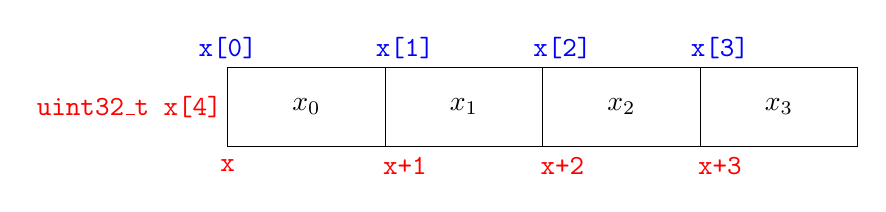
\begin{tikzpicture}
%	\def \xMax{10}
%	\def \xMin{-3}
%	\def \yMax{2}
%	\def \yMin{-4}
%	\draw[very thin,color=gray!15,step=.5] (\xMin,\yMin) grid (\xMax,\yMax);
%	
%	\foreach \i in {\xMin,...,-2,-1,1,2,...,\xMax}
%	\draw[gray] (\i,.1)--(\i,-.1) node[below] {$\i$};%x-axis
%	\foreach \i in {\yMin,-1,1,1,\yMax}
%	\draw[gray] (.1,\i)--(-.1,\i) node[left] {$\i$};%y-axis
	
	\def\n{3} 	   % Number of plaintexts (rows)
	\def\xstart{0} % Start point for plaintexts on the x-axis
	\def\ystart{0} % Start point for plaintexts on the y-axis
	\def\xgap{2} % Horizontal gap between bytes
	\def\ygap{1.5} % Vertical gap between rows
	
	\def\bytesA{{"\texttt{$x_0$}", "\texttt{$x_1$}", "\texttt{$x_2$}", "\texttt{$x_3$}"}}
	
	\foreach \i/\rowbytes in {1/\bytesA} {
		\pgfmathsetmacro{\y}{\ystart - \i * \ygap}
		
		% Draw each byte in the row inside a box
		\foreach \j in {1, ..., 4} {
			\pgfmathsetmacro{\x}{\xstart + (\j-1) * \xgap}
			\ifnum\j=1
			\node[draw, rectangle, minimum width=2cm, minimum height=1cm] 
			at (\x, \y) {\pgfmathparse{\rowbytes[\j-1]}\pgfmathresult};
			\else
			\node[draw, rectangle, minimum width=2cm, minimum height=1cm] 
			at (\x, \y) {\pgfmathparse{\rowbytes[\j-1]}\pgfmathresult};
			\fi
		}
	}

	\node[red] at (-2.25,-1.5) {\texttt{uint32\_t x[4]}};
	\node[red] at (-1,-2.25) {\texttt{x}};
	\node[red] at (1.25,-2.25) {\texttt{x+1}};
	\node[red] at (3.25,-2.25) {\texttt{x+2}};
	\node[red] at (5.25,-2.25) {\texttt{x+3}};
	
	\node[blue] at (-1,-.75) {\texttt{x[0]}};
	\node[blue] at (1.25,-.75) {\texttt{x[1]}};
	\node[blue] at (3.25,-.75) {\texttt{x[2]}};
	\node[blue] at (5.25,-.75) {\texttt{x[3]}};
\end{tikzpicture}
\end{document}